\documentclass[main.tex]{subfiles}
\begin{document}

\chapter{Quantum Information}

\section{The basics}

\paragraph{Qubit}

It can be physically realized with any two-state system.
It is a complex superposition of \(\ket{0} \) and \(\ket{1} \). Thanks to normalization and \(U(1)\) gauge invariance (a ket is defined up to a phase) we can always make \(\ket{0} \)'s coefficient real and \(\in [0,1]\): the ket can always be written as

\begin{equation} \label{eq:qubit}
    \ket{\psi} = \cos(\frac{\theta}{2}) \ket{0} + \sin(\frac{\theta}{2}) e^{ i  \varphi} \ket{1}
\end{equation}

with \(\varphi \in [0,2 \pi]\) and \(\theta \in [0, \pi]\): these can be interpreted as angles on a sphere. The fact that \(\theta\) is divided by two comes from the coordinates we choose in \(S^3 \subset \C^2\).

We can use an \(n\)-qubit system:

\begin{equation} \label{eq:n-qubit-state}
    \ket{\psi } = \sum _{i=0} ^{2^n-1} a_i \ket{i}
\end{equation}

where \(\ket{i} \) is a base state of the tensor product space of the \(n\) Hilbert spaces: \(\ket{i} = \ket{\alpha_0}_0 \otimes \ket{\alpha_1}_1 \otimes \dots \ket{\alpha_{n-1}}_{n-1} \); the \(\alpha_j\) are the components of the representation of \(i\) in binary: \(\alpha_0 \alpha_1 \dots \alpha_{n-1}\) (with \(\alpha_j =0,1\)). This is called the \emph{computational basis}.

We assume the state to be normalized: \(\sum _{i}  \abs{a_i} ^2 = 1 \)

\paragraph{Entanglement}

A state \(\ket{\psi } \) is called \emph{entangled} if there are no subsystem kets \(\ket{\psi _i} _i\), \(i = A, B\) such that \(\ket{\psi } = \ket{\psi _A} _A \otimes \ket{\psi _B} _B\).

\section{Quantum gates}
They are unitary trasformations: \(U: \H \rightarrow \H\), \(U ^\dag U = UU^\dag= \mathbb{1}\).

They can be decomposed into smaller gates, which are in general \(2n \times 2n\) complex unitary matrices, but we will usually just use \(n=1, 2\).

If two gates are represented by \(2 \times 2\) matrices, indexed in the computational basis as \(A_i ^j\) and \(B_k^l\) with \(i, j, k, l = 0,1\),  then their tensor product will be

\begin{equation}
    [A_i^j B_k^l] = [A \otimes B]_i^j\,_k^l = [A \otimes B ] _M ^N
\end{equation}

where we grouped the indices \(ik = M\) and \(jl=N\), in order to write two-component fourth order tensors as four-dimensional order two matrices. What are \(M\) and \(N\)  then? \(i, j\) and so on are binary digits, so it is natural to interpret \(M\) and \(N\) as numbers between \(0\) and \(3\) written in binary.
Of course, this can be generalized to any order, keeping the same pattern, and be applied to vectors as well.

\paragraph{Hadamard} \label{par:hadamard}
It is a \emph{one-qubit gate} which switches from the computational basis to the eigenstates of \(\sigma_z\), which we call \(\ket{+} = H \ket{0} \propto \ket{0} +\ket{1}   \) and \(\ket{-} = H \ket{1} \propto \ket{0} - \ket{1} \).

\begin{equation}
    H = \frac{1}{\sqrt{2} } \begin{pmatrix}
    1   & 1 \\
    1   & -1
    \end{pmatrix}
\end{equation}

We can also express it, for the basis states, as \(H \ket{x} = \sqrt{1/2} \sum _{y=0}^1 (-)^{xy} \ket{y}  \).

\paragraph{Phase}
It is a \emph{one-qubit gate} which  gives a phase to a state: applying it to a generic qubit, written as \eqref{eq:qubit}, we get \(R_z(\delta) \ket{\psi} =  \cos(\theta/2) \ket{0} + \exp(i(\varphi+\delta)) \sin(\theta/2)\ket{1}\).

\begin{equation} \label{eq:phase-gate}
    R_z (\delta) = \exp(i \delta \sigma_z) = \begin{pmatrix}
    1   & 0 \\
    0   & \exp(i \delta)
    \end{pmatrix}
\end{equation}

\paragraph{Control not} \label{par:cnot}
It is a \emph{two-qubit gate}  which cannot be written as a tensor product of one-qubit gates.

\begin{equation}
    \text{CNOT} = \begin{pmatrix}
    1   &  0 &   &  \\
      0 & 1  &   &  \\
       &   & 0  & 1 \\
       &   & 1  & 0
    \end{pmatrix}
\end{equation}

It generates entanglement: let us apply it to the separable state \(\alpha \ket{00} + \beta \ket{10} \): it returns \(\alpha \ket{00} + \beta \ket{11} \), which is entangled.

\paragraph{Control phase}

It is a \emph{two-qubit gate}:

\begin{equation}
    \text{CPHASE}(\delta) = \begin{pmatrix}
    \mathbb 1   & 0 \\
    0   & R_z(\delta)
    \end{pmatrix}
\end{equation}

where we used the phase gate \eqref{eq:phase-gate}.

\begin{bluebox}
It can be written as \(\text{CPHASE} (\delta) = [\mathbb 1 \otimes R_z(\delta/2)] [\text{CNOT}] [\mathbb 1 \otimes R_z(-\delta/2)] [\text{CNOT}] [ R_z(\delta/2) \otimes\mathbb 1 ]\): the steps  (multiplying from right to left, starting from just \([ R_z(\delta/2) \otimes\mathbb 1 ]\)) are as follows:

\begin{multline}
    \begin{pmatrix}
    1   &   &   &  \\
       & 1  &   &  \\
       &   & e^{i \delta/2}  &  \\
       &   &   & e^{i \delta /2}
    \end{pmatrix}
\rightarrow
    \begin{pmatrix}
    1   &   &   &  \\
       & 1  &   &  \\
       &   &  & e^{i \delta/2}  \\
       &   &   e^{i \delta /2} &
    \end{pmatrix}
\rightarrow
    \begin{pmatrix}
    1   &   &   &  \\
       & e^{-i \delta/2}  &   &  \\
       &   &  & e^{i \delta/2}  \\
       &   &   1 &
    \end{pmatrix}
\rightarrow
\\
\rightarrow
    \begin{pmatrix}
    1   &   &   &  \\
       & e^{-i \delta/2}  &   &  \\
       &   &  1 &  \\
       &   &    & e^{i \delta/2}
    \end{pmatrix}
\rightarrow
    \begin{pmatrix}
    1   &   &   &  \\
       & 1  &   &  \\
       &   &  1 &  \\
       &   &    & e^{i \delta}
    \end{pmatrix}
\end{multline}
\end{bluebox}

\begin{bluebox}
We can get any state \(\ket{\psi }\) written as \eqref{eq:qubit} with Hadamard and phase-shift:

\begin{subequations}
\begin{align}
  \ket{\psi }  &= R_z(\pi/2 + \varphi) H R_z(\theta) H\ket{0}  \\
  &= \frac{1}{2} \begin{pmatrix}
    1 + e^{i \theta} \\
     i  \qty(e^{i \varphi}  - e^{i (\theta + \varphi)})
  \end{pmatrix}  \\
  &= \label{eq:sub-gate-phase}
  \frac{1}{2} \begin{pmatrix}
    e^{i \theta /2} + e^{-i \theta /2} \\
    i^{-1} \qty(e^{i \theta/2} - e^{-i \theta/2}) e^{i \varphi}
\end{pmatrix}  \\
 &= \begin{pmatrix}
 \cos(\theta/2)  \\
 \sin(\theta/2) e^{i \varphi}
 \end{pmatrix}
\end{align}
\end{subequations}

where in the step \eqref{eq:sub-gate-phase} we used the fact that a quantum state is only defined up to a phase, and multiplied by \(\exp(-i \theta/2) \).
\end{bluebox}


\paragraph{Binary function unitarity}

In general a function \(f: \qty{0,1}^n \rightarrow \qty{0,1}\) will not be injective, therefore it will not be unitary. In order to represent it as unitary we must "carry over" the input:

\begin{equation}
    U_f \ket{x} \ket{0} = \ket{x} \ket{f(x)}
\end{equation}

in order to have a more general trasformation we define it for arbitrary input on the second system:

\begin{equation}
    U_f \ket{x} \ket{y} = \ket{x} \ket{y \oplus f(x)}
\end{equation}

where \(\oplus\) is bitwise XOR.

\paragraph{Parallelism}

We can do lots of computation with a single gate: say we have a state like \eqref{eq:n-qubit-state}, then

\begin{equation}
    U_f \sum _{x=0}^{2^n-1} a_x \ket{x} \ket{y}  = \sum _{x=0}   ^{2^n-1} a_x \ket{x} \ket{y \oplus f(x)}
\end{equation}

For this to be really different from classical computing, however, a significant portion of the \(2^n\) coefficients \(a_x\) must be nonzero. We now will show how to produce the state in which they are all equal to \(2^{-n/2}\), assuming we can produce \(\ket{0} ^{\otimes n}\). We apply a \nameref{par:hadamard} gate to every qubit, which carries a normalization and a factor of \((-)^{x_i y_i}\), so we get:

\begin{equation}
    H ^{\otimes n} \ket{x} = \frac{1}{\sqrt{2^n} } \sum _{y=0}   ^{2^n -1} (-)^{x\cdot y} \ket{y}
\end{equation}

And the desired state can be found by setting \(x = 0\). Do note that while this looks "entangled" we found it by applyng single-qubit gates: it is still separable (we can see this from the fact that its density matrix has the same value in every entry, so its rank is 1).

\paragraph{No cloning}

A  \emph{general}  cloning unitary operator would look like: \(U \ket{x} \ket{0} = \ket{x} \ket{x} \).
Let us assume we have one, and let us apply it to two different states: \(A = U\ket{\psi}\ket{0}=\ket{\psi} \ket{\psi }  \) and \(B = U\ket{\varphi} \ket{0} = \ket{\varphi} \ket{\varphi} \). Now, let us compute the scalar product of \(A\) and \(B\):

\begin{subequations}
\begin{align}
  A \cdot B &= \bra{\psi} \bra{0} U^\dag  U\ket{\varphi} \ket{0}  \\
  &= \braket{\psi}{\varphi} \braket{0}{0} U^\dag U  \\
  &= \braket{\psi}{\varphi}
\end{align}
\end{subequations}

but also

\begin{subequations}
\begin{align}
  A \cdot B &= \bra{\psi} \bra{\psi}  \ket{\varphi} \ket{\varphi}   \\
  &= \braket{\psi}{\varphi}^2
\end{align}
\end{subequations}

and in general \(\braket{\psi}{\varphi} \neq 0,\pm 1\), so we found a contradiction. Note that we \emph{can} create a partial cloning machine which works only on the basis states of some basis: we extend by linearity the desired cloning. If we want to clone the computational basis, the gate is the CNOT (see \Nameref{par:cnot}).

\begin{bluebox}
  Alternative proof: apply \(U (\ket{x} + \ket{y}) \otimes \ket{0} = (\ket{x} + \ket{y}) ^{\otimes 2} \) (a separable state), but \(U\) must be linear, so \(U (\ket{x} + \ket{y}) \otimes \ket{0} = \ket{x} \ket{x} + \ket{y} \ket{y} \), generally an entangled state.
\end{bluebox}

\section{Miscellaneous concepts}

\subsection{Algorithmic complexity}

We can distinguish algorithms by how many resources (computation time, RAM, ...) they require:

\begin{enumerate}
    \item \(P\): classical polynomial time;
    \item \(NP\): classical nondeterministic polynomial time: there exists a nondeterministic Turing machine\footnote{Same as a regular Turing machine, except that in a certain configuration it can have different actions, and in a certain sense it ``tries them all''.} which finds the solution in polynomial time --- the solution can thus be verified in polynomial time;
    \item \(NP-\text{hard}\): problems to which every \(P\) problem can be reduced in polynomial time;
    \item \(NPC\): \(NP\) problems which are also \(NP-\text{hard}\);
    \item \(BPP\): bounded error probabilistic polynomial: it can give us the correct answer in polynomial time with probability \(\P>1/2\).
    \item \(BQP\): bounded error quantum polynomial: it is a quantum algorithm which can give us the correct answer in polynomial time with probability \(\P>1/2\).
\end{enumerate}

Surely \(P \subseteq BPP \subseteq BQP\). We are not sure whether \(BQP \subseteq BPP\).

\subsection{Fidelity}

We introduce a notion of distance between states:

\begin{equation}
    F = \abs{\braket{\psi_1}{\psi_2} }^2
\end{equation}

\(F\) is monotonous in \(\norm{\ket{\psi_1} - \ket{\psi _2} }_2\).
\(F\) is also the \(\cos^2(\theta/2) \), where \(\theta\) is the angle between the two vectors in Bloch space.

\begin{bluebox}
  Let us prove these two statements: first of all notice that \(\norm{\ket{\psi_1} - \ket{\psi _2} }_2 = \sqrt{2 - 2 \Re \braket{\psi_1}{\psi_2}}\).
  Now, the scalar product \(\braket{\psi_1}{\psi_2}\) is in general a complex number but we can rotate the starting functions by an arbitrary phase, making it real and positive. So we get \(\Re \braket{\psi_1}{\psi_2} = \abs{\braket{\psi_1}{\psi_2}}  = \sqrt{F} \). Then, we can see that

  \begin{equation} \label{eq:norm-of-difference-fidelity}
    \norm{\ket{\psi_1} - \ket{\psi _2} }_2 = \sqrt{2(1-\sqrt{F})}
  \end{equation}

  Now, we want to prove \(F = \cos^2(\theta/2) \): let \(U\) be a unitary transformation which maps \(\ket{\psi _1} \) to \(\ket{0}\). We can rewrite \(F = \abs{\bra{\psi_1} U^\dag U \ket{\psi_2}}^2\). We can expand the applications of \(U\) to the vectors to get \(\abs{\bra{0} \qty(\alpha \ket{0} + \beta \ket{1} ) }^2\).

  Now, since states are always defined up to a phase, we can pick \(\alpha\) to be real and positive. Then we have put the state \(U \ket{\psi_1}\) in the canonical form \eqref{eq:qubit}, and the result follows.
\end{bluebox}

\begin{figure}
    \centering
    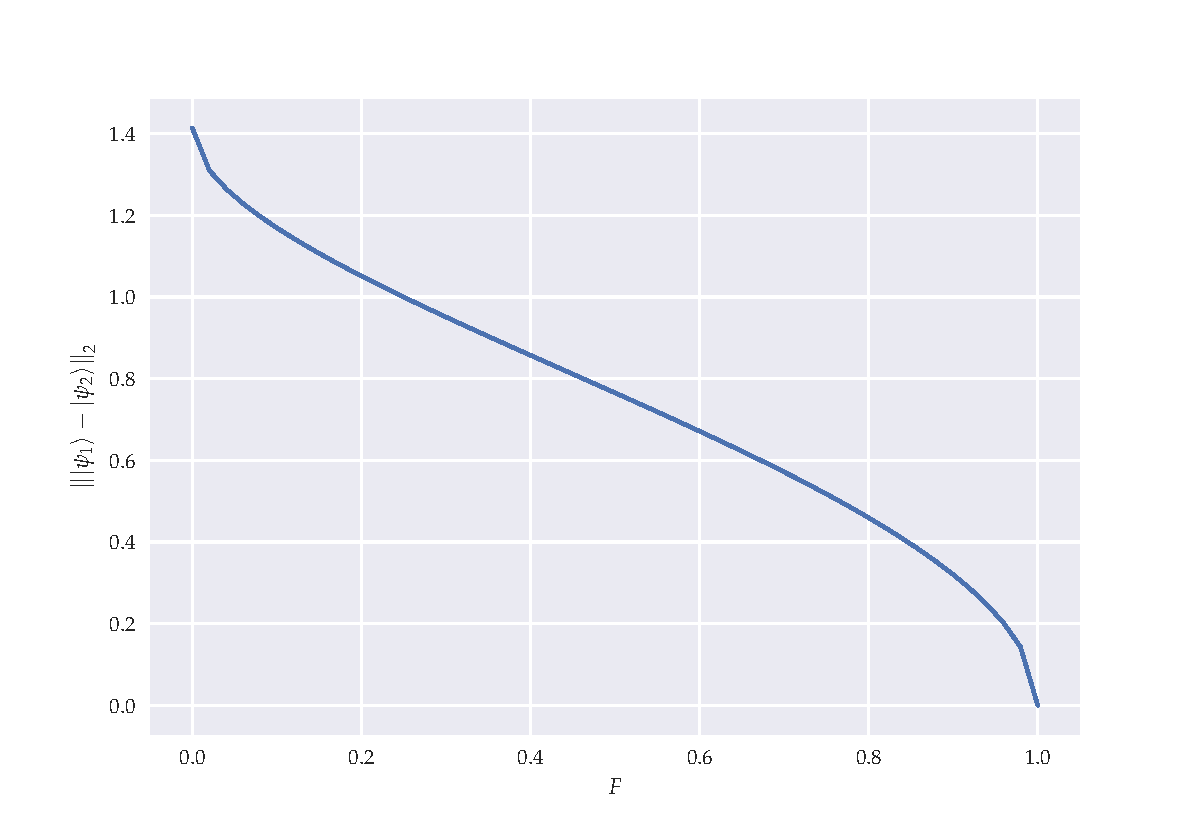
\includegraphics[width=0.7\textwidth]{figures/Fidelity.pdf}
    \caption{Norm of difference vs fidelity: a plot of equation \eqref{eq:norm-of-difference-fidelity}}
    \label{fig:fidelity}
\end{figure}

\section{Quantum teleportation}

It is possible to clone a generic quantum state \(\ket{\psi } = \alpha \ket{0} + \beta \ket{1}  \) assuming we start with two entangled qubits, one in the starting location and one at the destination: so, if these two qubits are called \(A\) and \(B\) and the state we want to transmit is in subsystem \(C\), we start with

\begin{equation}
    \qty(\frac{\ket{00} + \ket{11} }{\sqrt{2} })_{AB} \otimes \ket{\psi}_C
\end{equation}

The protocol is this:

\begin{enumerate}
    \item Apply the gate \(\text{C}_C\text{NOT}_A\); \label{step:cnot}
    \item apply the gate \(H_C\); \label{step:hadamard}
    \item measure \(A\) and \(C\) in the computational basis: call the result \(x\);
    \item apply a gate \(V_x\), selected according to table \ref{tab:teleportation-gate}, to \(B\).
\end{enumerate}

\begin{table}[H]
    \centering
    \begin{tabular}{c|c}
        \(x\) & \(V_x\) \\
        \hline
        00 & \(\mathbb 1\) \\
        01 & \(\sigma_z\) \\
        10 & \(\sigma_x\) \\
        11 & \(\sigma_z \sigma_x\)
    \end{tabular}
    \caption{Possibilities for gate \(V_x\). }
    \label{tab:teleportation-gate}
\end{table}

\begin{greenbox}
  Possibly, when Montangero wrote \(AC=01\) he meant \(A=1\) and \(C=0\).
\end{greenbox}

We can realize all of this with the gates \(\text{CNOT}\), Hadamard and \(\sigma_z\) (we can recover \(\sigma_x\) as \(\sigma_x = H \sigma_z H\).

\section{Quantum interferometry}

\paragraph{Beam splitter}

We call the sides of the BS \(A\) and \(B\), and denote the absence or presence of light on either side by \(\ket{0,1} _{A, B}\). Then the action of the beam splitter is unitary and can be represented in the partial basis \(\ket{0}_A \otimes \ket{1} _B , \ket{1}_A \otimes \ket{0} _B\) as

\begin{equation}
    U_{BS} = \frac{1}{\sqrt{2} }
    \begin{pmatrix}
    1   & i \\
    i   & 1
    \end{pmatrix}
\end{equation}

Note that \(U_{BS}^2 = i\sigma_x\) in the BS-side basis: if we build a Mach-Zender interferometer, that is, we chain two beam-splitters, the light from the two paths interferes and we get some only on one side of the BS (the side opposite of the starting one).

\paragraph{Bomb detection}

If we block one of the paths between the detectors, around half of the time the light will hit this obstacle (our `bomb'). Around half the time it will go to the second BS, and then a quarter of the time it will be detected on either side of the BS. On the other hand, if there is no obstacle, we will see photons \emph{only} on a certain side of the final BS.

So around \(\frac[i]{1}{4} \) of the time we will have detected the bomb without the photon actually \emph{having been there}.

\section{Zeno effect} \label{sec:zeno}

We will with \(\hbar=1\).
We look of the \emph{survival probability} with which we will retain our starting state: if our evolution operator is \(U = \exp(-iHt) \), this probability is \(\P = A^*A\), where \(A = \braket{\psi_0}{\psi (t)} \) and \(\ket{\psi (t)} = U \ket{\psi _0} \).

How does this probability look like for small \(t\)? We can expand, for a small \(\delta{t}\):

\begin{equation}
    U \sim \mathbb 1 -i H \delta{t} - H^2 \delta t^2
\end{equation}

then we will have

\begin{equation}
    A = \bra{\psi_0}  \qty(\mathbb 1 -i H \delta{t} - H^2 \delta t^2) \ket{\psi_0}
    = 1 -i \expval{H}_0 \delta{t} - \frac{1}{2}  \expval{H^2} _0 \delta t^2
\end{equation}

so we can calculate \(\P\):

\begin{equation} \label{eq:zeno-probability}
    \P = \abs{1 -i \expval{H}_0 \delta{t} - \frac{1}{2} \expval{H^2} _0 \delta t^2}^2
    = 1 - \delta t^2 \qty(\expval{H^2} _0 - \expval{H}_0^2)
\end{equation}

Equation \eqref{eq:zeno-probability} is accurate to the order \(\delta t^3\), since we only ignored a fourth order term. The term multiplying \(\delta t^2\) can be interpreted as the inverse of a characteristic time:

\begin{equation}
    \tau = \frac{1}{\sqrt{\expval{H^2} _0 - \expval{H}_0^2}} = \frac{1}{\Delta H _0}
\end{equation}

\paragraph{Repeated measurements}

If we measure some observable with \(\ket{\psi _0}\) as an eigenspace, a fraction \(\frac[i]{t^2}{\tau^2} \) of the time we will get something different from \(\ket{\psi _0} \).

So, if in a long time \(t\) we measured \(N\) times, the probability of the system having remained in the original state is at least \(\P (t) \geq \P^N(\frac[i]{t}{N} )\): we consider the case in which the system remained in the state for \emph{all} the measurements. The latter pertains to a small time so we can apply equation \eqref{eq:zeno-probability}:

\begin{equation}
    \P \geq \P^N\qty(\frac{t}{N}) = \qty(1- \frac{t^2}{N^2 \tau^2} )^N
\end{equation}

if we fix the inverse of the measurement rate \(\frac[i]{N}{t} = R\) this becomes \(\P \geq x^t = \exp(t \log x) \), with \(x = \qty(1 - \frac[i]{1}{R^2\tau^2})^R\), so \(\log x =  R \log(1- \frac[i]{1}{R^2 \tau^2} ) < 0\). So, we call \(-\log x = \gamma_{\text{eff}}>0 \): then

\begin{equation}
    \P \geq e^{-\gamma _{\text{eff}} t }
\end{equation}

Note that as \(R \rightarrow \infty\), \(\gamma _{\text{eff}} \sim R^{-1}\tau^{-2}\).

\paragraph{An example of nonunitary evolution}

We consider a Hamiltonian like \(H = \Omega \sigma_x \), which might be that of a spin-$1/2$ particle, polarized along \(z\), in a magnetic field along \(x\). Say our system starts at \(\ket{\psi _0}  = \ket{0} \). Then the evolution looks like

\begin{equation}
    \exp(-iHt) \ket{0} = \cos(\Omega t) \ket{0} -i \sin(\Omega t) \ket{1}
\end{equation}

We can calculate the quantities from section \ref{sec:zeno}: \(A = \cos(\Omega t) \) and \(\P = \cos^2(\Omega t)\), for small \(t\):  \(\P \sim 1- \Omega^2  t^2\). We recognise the expression for the Zeno time: in this case \(\tau = \Omega^{-1}\)

Let us introduce the nonunitary part: we change \(H\) to

\begin{equation} \label{eq:interaction-hamiltonian}
    H _{\text{int}}  = \begin{pmatrix}
    -iV \\
    \Omega  \\
    0    \\
    +iV
    \end{pmatrix}
    \cdot
    \begin{pmatrix}
    \mathbb 1 \\
    \sigma_x  \\
    \sigma_y  \\
    \sigma_z
    \end{pmatrix}
    =
    -iV \mathbb 1 + \vec{h} \cdot \vec{\sigma}
    =
    \begin{pmatrix}
    0   & \Omega   \\
    \Omega  & -2iV
    \end{pmatrix}
\end{equation}

to represent interaction with a second lower-energy system, to which our first one can decay \emph{if it is in the state \(\ket{1}\)}. Can we get a Zeno-like effect with this kind of interaction, and without \emph{measuring} anything?
The evolution of this new Hamiltonian will look like

\begin{equation}
    \exp(-itH) = e^{-tV} \exp(-it \vec{h} \cdot \vec{\sigma} ) = e^{-tV} \qty(\cosh(h t)\mathbb 1 -i \frac{\vec{\sigma} \cdot \vec{h} }{h} \sinh(ht) )
\end{equation}

where \(h = \sqrt{ V^2 - \Omega^2} \in \R\), since we assume the coupling is strong (\(V \gg \Omega\)). This comes from the fact that for a unit vector \(\vec{n} \): \((\vec{n} \cdot \vec{\sigma})^n = \mathbb 1  )\) if \(N\) is odd, \(\vec{n} \cdot \vec{\sigma} \) otherwise.

So, we can compute \(A = \expval{U} _0\):

\begin{equation}
    A = \frac{1}{2} \qty(1 + \frac{V}{h})e^{-(V-h)t}+
    \frac{1}{2} \qty(1 - \frac{V}{h})e^{-(V+h)t}
\end{equation}

\(V\) is close to \(h\) but slightly larger, so both the exponentials' arguments are negative.

For large times we can discard the quickly-decaying second exponential, and be left with

\begin{equation}
    \P = \abs{\frac{1}{2} \qty(1 + \frac{V}{h})e^{-(V-h)t}}^2
    \sim \qty(1 + \frac{\Omega^2}{2 V^2}) \exp(-t \frac{\Omega^2}{V})
\end{equation}

So, weird normalizations for small times aside, \(\gamma _{\text{eff}} = \Omega^2 /V \), but \(Omega = \tau^{-1}\), so \(V = R\), the `rate of observation': the stronger the coupling, the more the other system influences ours.

\section{Non-unitary evolution}

It happens when the particle can escape the system; for example in optical systems there can be a complex index of refraction. The Hamiltonian will look like

\begin{equation}
    H = H_0 - iV \mathbb 1
\end{equation}

where \(V \in \R^+\). The unitary evolution has an \(i\) multiplying the Hamiltonian, so we get a decreasing real exponential.

We will have \(A \sim 1 -V \delta t + O(\delta t^2)\), so \(\P  \sim 1 - 2V \delta t + O(\delta t^2)\): the first derivative is nonzero!

\paragraph{An example of a nonhermitian Hamiltonian}

We consider a system and its environment together:

\begin{equation}
    H = \underbrace{\Omega \sigma_x}_{\substack{\text{system}}}  + \underbrace{\int   \dd{\omega} \dyad{\omega}}_{\substack{\text{environment}}} + \underbrace{\sqrt{\frac{\Gamma}{2 \pi}} \int   \dd{\omega} g(\omega) \qty(\ketbra{-}{\omega} + \ketbra{\omega}{-}  )  }_{\substack{\text{interaction}}}
\end{equation}

Where \(\sigma_x\) is meant to be in the \(\ket{-}, \ket{+}  \) basis. Now, let us take a generic state \(\ket{\psi } = x(t) \ket{-} + y(t) \ket{+} + \int \dd{\omega} z(\omega, t) \ket{\omega} \).

We will write the Schrödinger equation for the evolution of \(x\), \(y\) and \(z\) and show that, if we just consider the first two, the effective Hamiltonian looks like the one in \eqref{eq:interaction-hamiltonian}.

The system so solve can be separated into

\begin{subequations}
\begin{align}
  i \dot{x} &= \Omega y \\
  i \dot{y} &= \Omega x +\sqrt{\frac{\Gamma}{2 \pi}} \int z \dd{\omega}   \\
  i \dot{z} &= \omega z +\sqrt{\frac{\Gamma}{2 \pi}} y
\end{align}
\end{subequations}

In can be readiliy verified that, with starting conditions \(x=1\), \(y=z=0\), we have

\begin{equation}
    z(\omega, t) = -i \sqrt{\frac{\Gamma}{2 \pi}} \int _{0}   ^{t} \dd{\tau} y(\tau) e^{-i \omega (t-\tau)}
\end{equation}

so we substitute into the equation for \(y\)

\begin{equation}
    i \dot{y} = \Omega x  -i\frac{\Gamma}{2 \pi} \int \dd{\omega} \int _{0}   ^{t} \dd{\tau} y(\tau) e^{-i \omega (t-\tau)}
\end{equation}

but \(\int   \dd{\omega} e^{-i \omega (t- \tau)} = 2 \pi \delta(t- \tau)\): so

\begin{equation}
    i \dot{y} = \Omega x  -i\Gamma y(t) /2
\end{equation}

The factor \(1/2\) comes from the fact we integrated a \(\delta\) on the \emph{boundary} of the domain.
We can combine the results into

\begin{equation}
    i \dv{}{t} \begin{pmatrix}
    x \\
    y
    \end{pmatrix}
    = \begin{pmatrix}
    0   & \Omega     \\
     \Omega  & -i \Gamma /2
    \end{pmatrix}
    \begin{pmatrix}
    x \\
    y
    \end{pmatrix}
\end{equation}

\section{Implementation of quantum gates}

We want to implement a NOT gate (\(\sigma_x\)): we use a spin-$1/2$ particle, and two magnetic fields described by  a Hamiltonian

\begin{equation}
    H = - \mu \qty(B_0 \sigma_z + B_1 \qty(\cos(\omega t) \sigma_x + \sin(\omega t)\sigma_y  ))
\end{equation}

So the zeroth field is fixed on \(z\), while the other rotates around the \(z\) axis staying on the \(xy\) plane.

\begin{greenbox}
  TODO
\end{greenbox}

\section{Density matrices}

Say we have a generic observable \(\hat{A} = \sum _{i}  a_i \dyad{a_i} \), and our has a probability \(p_i\) of being in the state \(\ket{\psi_i}\): of course we must have \(\sum _{i}  p_i = 1 \). Then, we want to compute the expectation value \(\expval{A} \) in this ``mixed'' state: it will look like

\begin{subequations}
\begin{align}
   \expval{A} &= \sum _{i,k} p_i a_k \braket{\psi_i}{a_k}\braket{a_k}{\psi_i}   \\
   &= \sum _{i,j,k}  p_i a_k  \bra{a_k}\qty(\ketbra{a_j}{a_j})\ket{\psi_i} \braket{\psi_i}{a_k}  \\
   &= \sum _{k} \bra{a_k} \qty(\sum_j \underbrace{a_k}_{\substack{k\equiv j\text{ since it is }\\ \text{multiplied by }\delta_{jk}}}  \dyad{a_j} ) \qty(\sum_i p_i \dyad{\psi_i} ) \ket{a_k} \\
   &= \Tr \qty(A \rho) = \Tr \qty(\rho A)
\end{align}
\end{subequations}

So, we have defined

\begin{equation}
    \rho \defeq \sum _{k} p_k  \dyad{\psi_k}
\end{equation}

\paragraph{Properties}

\begin{enumerate}
    \item \(\Tr \rho = 1\)
    \item \(\rho = \rho^\dag\)
    \item \(\rho \geq 0\)
    \item \(\Tr \rho^2 \leq 1\)
\end{enumerate}

These can be deduced from writing the matrix elements \(\rho _{ij} = \bra{i} \rho \bra{j} \) in an ON basis, or by noticing that \(\rho \) is a positively-weighted sum of projectors, each of which is self-adjoint.

The first one needs the components approach, I think: \(\rho_{ii} = \sum _{ik}  \abs{\braket{\psi_k}{i} }^2 =1 \) since they are the components in a basis of a normalized ket.

The last property can be seen by noticing that \(\rho\) is self-adjoint, so it has an orthonormal basis: then squaring it is easy, and all the coefficients are such that \(p_i^2 \leq p_i\).

\paragraph{Time evolution of a density matrix}

How does \(\rho\) evolve? If we have \(U\), we can write the evolution by linearity as

\begin{equation}
    \rho(t) = \sum _{k} p_k  U\dyad{\psi_k}U^\dag =  U \rho_0 U^\dag
\end{equation}

If instead we wish to look at the differential formulation, starting from \(i \hbar \ket{\dot{\psi}_k} = H \ket{\psi_k}\) and its adjunct \(-i \hbar \bra{\dot{\psi}_k} =  \bra{\psi_k} H\) we get

\begin{equation}
    \dv{}{t} \rho(t) =  \sum _{k} p_k  \dv{}{t} \qty(\dyad{\psi_k})
    = \frac{1}{i \hbar} \sum _{k} p_k  \qty(H \dyad{\psi_k} - \dyad{\psi_k}H)
    = \frac{[H, \rho]}{i \hbar}
\end{equation}

\paragraph{Pure states}

A density matrix is a \emph{pure state} if it has only one component, in the sense that: \(\rho = \dyad{\psi} \). The following are equivalent:

\begin{enumerate}
    \item \(\rho \) is a density matrix;
    \item \(\rho\) has rank 1;
    \item \(\Tr \rho^2 = 1\).
\end{enumerate}

The quantity \(\Tr \rho^2\) is called the \emph{purity}, and is surely greater than \(1/d\), \(d\) being the dimension of the Hilbert space (consider \(\rho = d^{-1} \mathbb 1\)).

\paragraph{Examples of density matrices}

For a single pure qubit:

\begin{equation}
    \rho = \dyad{\psi} = \begin{pmatrix}
    \cos^2(\theta/2)    & \cos(\theta/2) \sin(\theta/2) e^{-i \varphi}    \\
     \cos(\theta/2) \sin(\theta/2) e^{i \varphi}  & \sin^2(\theta/2)
    \end{pmatrix}
\end{equation}

For a generic one-qubit mixed state:

\begin{equation}
    \rho = \frac{1}{2}\begin{pmatrix}
    1 \\
    x  \\
    y    \\
    z
    \end{pmatrix}
    \cdot
    \begin{pmatrix}
    \mathbb 1 \\
    \sigma_x  \\
    \sigma_y  \\
    \sigma_z
    \end{pmatrix}
    = \frac{1}{2} \begin{pmatrix}
     1+z  & x-iy \\
     x+iy  & 1-z
    \end{pmatrix}
\end{equation}

it can be shown by direct computation that in this case \(\Tr \rho^2 = \frac[i]{1}{2} (1+\abs{r}^2) \),where \(\vec{r} = (x, y, z) \): so the state is pure for \(\abs{\vec{r}}=1 \), and the purity is quadratic in \(\abs{\vec{r}}\).

We could also look at \(\det \rho = \frac[i]{1}{4} (1-\abs{r}^2)\) and see that it is zero when \(\abs{\vec{r} }=1 \), but that method seems less powerful...

\paragraph{Composite systems}

Say we have two Hilbert spaces 1 and 2, with their respective orthonormal bases \(\ket{i} \) and \(\ket{\alpha} \) respectively (let us work with finite-dimensional ones for simplicity).

Say we want to calculate the expectation value of an observable \(A_1\) on 1: we must write it as \(A_T = A \otimes \id_2\).
Of course, our density matrix will also have four indices.
Then

\begin{equation}
    \expval{A} = \Tr \qty(\rho A_T)
    = \sum _{k \gamma} \bra{k \gamma}
    \qty(\sum _{ij \alpha \beta} \rho_{i \alpha}^{j \beta}  \ketbra{i \alpha}{j \beta})
    %\qty( A \otimes \id_2)
    \qty(\sum_{mn \sigma \xi} A_m^n \delta_ \sigma^ \xi \ketbra{m \sigma}{n \xi})
    \ket{k \gamma}
\end{equation}

So we can make the sums implicit,  the components of \(A\) explicit, and simplify some \(\delta\)s:

\begin{equation}
    \Tr \qty(\rho A_T)
    = \delta_k^i \delta_\gamma ^\alpha
    \rho_{i \alpha}^{j \beta}
    \delta_j ^m \delta_\beta^\sigma
    A_m^n \delta_ \sigma^ \xi
    \delta_n^k \delta_\xi^\gamma
    %= \rho_{i \alpha}^{j \beta} A_m^i \delta_{\beta}^\alpha  \delta^m_k   \delta_j^k
    = \rho_{i \alpha}^{j \alpha} A_j^i
\end{equation}

The simplifications are easier to understand by writing the index equivalencies:
\(m \equiv j\), \(i \equiv k \equiv n\) and \(\alpha \equiv \gamma \equiv \xi \equiv \sigma \equiv \beta\).

The trace with a simple one-subsystem density matrix, with the same one-subsystem observable \(A\), would look like

\begin{equation}
    \Tr \qty(\rho A) = \rho_i ^j A_j^k \delta_k ^i = \rho_i^j A_j^i
\end{equation}

So it becomes clear that we can use the traced matrix \(\rho_{i \alpha}^{j \alpha} \defeq (\rho_1)_i^j\) as a \emph{reduced density matrix} for the first subsystem.

We can write this in index-free notation as

\begin{equation} \label{eq:reduced-density-matrix}
    \rho_1 = \Tr_2 \rho
\end{equation}

Note that even when \(\rho\) is a pure state, if we trace out a subsystem it can become mixed: this can be seen with \(\rho = \frac[i]{1}{2} (\ket{00} + \ket{11})(\bra{00} + \bra{11})\), whose \(\rho_1 = \frac[i]{1}{2} (\dyad{0} + \dyad{1})\).

\section{Correlations}

We want to characterize quantum observables \(x\) and \(y\). Let us start by defining the standard deviation:

\begin{equation}
    \sigma_x = \sqrt{\expval{\qty(x - \expval{x} )^2}}
\end{equation}

So, we can define the covariance between two variables:

\begin{equation}
    C_{xy} = \frac{\expval{(x - \expval{x}) (y - \expval{y} )}}{\sigma_x \sigma_y}
    = \frac{\expval{xy} - \expval{x} \expval{y} }{\sigma_x \sigma_y}
\end{equation}

(Unless \([x,y]=0\) this is not the same as \(C_{yx}\)!)

\section{Schmidt decomposition}

Let us take a generic state in a two-subsystem system: \(\ket\psi = \sum _{i, \alpha} c_{i \alpha} \ket{i}_A \ket{ \alpha}_B \). In general, this will be a superposition of \(\dim A \dim B\) states. Schimdt  says we can write it as

\begin{equation}
    \ket{\psi}
    = \sum _{i=1} ^k \sqrt{p_i}  \ket{i}_A \ket{\alpha(i)} _B
\end{equation}

where \(k\) is called the \emph{Schmidt rank}, and the \(\ket{\alpha(i)} \) are orthormal. Also, \(p_i \geq 0\) and \(\sum _{i} p_i = 1 \).

How do we get this? We start from our generic state and rewrite it:

\begin{subequations}
\begin{align}
  \ket\psi &=  \sum _{i, \alpha} c_{i \alpha} \ket{i}_A \ket{ \alpha}_B  \\
  &= \sum _{i}  \ket{i} \qty(\sum _{\alpha} c_{i \alpha} \ket{\alpha})  \\
  &= \sum _{i}  \ket{i} \ket{\widetilde{\alpha} (i) } \label{eq:two-subsystem-schmidt-state-nonnormalized}
\end{align}
\end{subequations}

This seems fine,  but the \(\ket{\widetilde{\alpha}(i) } \) do not have the properties we want: they are not orthonormal.
Let us use equation \eqref{eq:reduced-density-matrix}, with an explicit one-subsystem matrix, and set it equal to the density matrix of \eqref{eq:two-subsystem-schmidt-state-nonnormalized}.

\begin{subequations}
\begin{align}
  \sum _{i} p_i \dyad{i}   &= \Tr_2 \qty(\sum _{i,j}  \ket{i} \ket{\widetilde{\alpha} (i)} \bra{j} \bra{\widetilde{\alpha }(j)})  \\
  &= \sum _{\gamma} \bra{\gamma}  \qty(\sum _{i,j}  \ket{i} \ket{\widetilde{\alpha} (i)} \bra{j} \bra{\widetilde{\alpha }(j)}) \ket{\gamma}  \\
  &= \sum _{i,j}  \ket{i}\bra{j}
  \qty(\bra{\widetilde{\alpha} (i)} \qty(\sum _\gamma \dyad{\gamma})  \ket{\widetilde{\alpha }(j)})^*  \\
  &= \sum _{i,j}  \ket{i}\bra{j}
  \braket{\widetilde{\alpha} (j)}{\widetilde{\alpha} (i)}
\end{align}
\end{subequations}

So, in order for the equality to work it must be that \(\braket{\widetilde{\alpha} (j)}{\widetilde{\alpha} (i)} = p_i \delta_{ij}\). So, we can rewrite equation \eqref{eq:two-subsystem-schmidt-state-nonnormalized} with \(\ket{\widetilde{\alpha}(i) }  \rightarrow  \ket{\widetilde{\alpha} (i) } / \sqrt{p_i} \), which are orthonormal.
So, we get

\begin{equation}
    \ket{\psi} = \sum _{i} \sqrt{p_i}  \ket{i} \ket{\widetilde{\alpha} (i) }
\end{equation}

and the properties of the \(p_i\) are inherited from the one-subsystem matrix.

Note that the Schmidt rank is very susceptible to small perturbations.

\paragraph{Correletions for separable states}

A separable state can be written as \(\ket{\psi} = \ket{i}_A \ket{\alpha}_B\). If we have an observable on either system, then the correlation will be zero, since the averaging in \(\expval{x_Ay_B} \) will factor.

\paragraph{Purification} \label{par:purification}

If we have a generic state \(\rho = \sum _{i} p_i \dyad{i}  \), we can add a second subsystem in order to make it into a pure state: let us call the full density matrix \(\sigma = \dyad{\psi} \), which must equal \(\rho\) if we trace out the second system. The components of \(\sigma\) will look like \(\sigma_{i \alpha} ^{j \beta} = c_{i \alpha} c^*_{j \beta}\), \(c\) being the components of \(\ket{\psi } \) in the two-system basis.

\begin{subequations}
\begin{align}
    \rho &= \sum _{\gamma}  \bra{\gamma}
    \qty(\sum _{ij \alpha \beta} \sigma_{i \alpha} ^{j \beta} \ket{i \alpha} \bra{j \beta}   )
    \ket{\gamma}  \\
    &= \sum _{ij \alpha \beta} \sigma_{i \alpha} ^{j \beta} \ket{i} \bra{j} \braket{\beta}{\alpha}  \\
    \sum _{ij} \rho_{ij} \ketbra{i}{j} &= \sum_{ij \alpha \beta} c_{i \alpha} c^*_{j \beta} \delta_ \alpha ^ \beta \ketbra{i}{j}
\end{align}
\end{subequations}

So the equation to be solved is \(\rho_{ij} = c_{i \alpha} c_{j \alpha}^*\): these are \((\dim A)^2\) equations, and we have \((\dim B)^2\) parameters to tweak: so this can always be done with \(\dim B = \dim A\).

\section{Kraus representation}

How does a subsystem \(\rho_1\) of \(\rho = \rho_1 \otimes \dyad{G}_2 \) evolve? We are using a pure state for subsystem 2 but the construction will be general, since as we saw in \Nameref{par:purification} we can purify states.
We know that \(\rho(t) = U \rho U^\dag\), so:

\begin{equation}
    \rho_1(t) = \Tr_{2} \qty(U\qty(\rho_1 \otimes \dyad{G}_2 )U^\dag)
    = \sum _k \bra{k} U \ket{G} \rho_1 \bra{G} U^\dag \ket{k}
\end{equation}

so we define \(E_k = \bra{k} U \ket{G}\). Note that this is still a matrix, since we only contracted the subsystem 2 indices. These matrices obey \(\sum _{k}  E_k ^\dag E_k = \id\).
With this, we get

\begin{equation}
    \rho_1 (t) = \sum _{k} E_k \rho_1 E_k ^\dag
\end{equation}

This defines a \emph{superoperator} \(\mathcal S: \rho \rightarrow \sum _k E_k ^\dag E_k ^\dag \).

Because of how it was defined, \(\mathcal S\) has the following properties:

\begin{enumerate}
    \item it preserves self-adjointness; \label{item:superoperator-prop-1}
    \item it preserves the trace;\label{item:superoperator-prop-2}
    \item it preserves non-negativity.\label{item:superoperator-prop-3}
\end{enumerate}

The set of the \(\mathcal S\) also has a group structure, and \(\mathcal S^{-1}\) exists iff \(\mathcal S\) is unitary.

\paragraph{Kraus representations}

Any superoperator with properties \ref{item:superoperator-prop-1}, \ref{item:superoperator-prop-2} and \ref{item:superoperator-prop-3} it  can be written as

\begin{equation}
    \mathcal S (\rho) = \sum _k E_k \rho E_k ^\dag
\end{equation}

\section{Generalized measurements}

A generalized measurement is defined by a set of operators \(M_i\), such that \(\sum _i M_i ^\dag M_i = \id\). They represent the possible results of the measurement: the wavefunction is reduced to

\begin{equation}
    \frac{M_i \ket{\psi}}{\norm{M_i \psi}}
    \qquad
    \text{with probability}
    \qquad
    p_i=
    \norm{M_i \ket{\psi}}^2
    = \bra{\psi} M_i ^\dag M_i \ket{\psi}
\end{equation}

Note that the probabilities are normalized: \(\sum _i p_i = 1\).

If all the \(M_i\) are projectors (\(M_i = M_i ^\dag = M^2_i\)) then we get the usual Von Neumann projective measurements.

\paragraph{Naimark Theorem}

Generalized measurements are equivalent to projective measurements in a larger space: more specifically, a generalized measurement is equivalent to:

\begin{enumerate}
    \item Adding some ancillary qubits;
    \item evolving the whole system unitarily;
    \item taking a projective measurement.
\end{enumerate}

\subparagraph{Unitary characterization of Kraus evolution}

We have some Kraus evolution \(\rho \rightarrow \sum _{k}  E_k \rho E_k ^\dag \), with \(\sum _{k}  E_k ^\dag E_k = \id \).

Let us introduce a subsystem 2, with dimension the number of Kraus operators, and its orthonormal basis \(\ket{k} \), and the operator

\begin{equation}
    U \ket{\psi}_1 \ket{0}_2 \defeq \sum _{k}  E_k \ket{\psi}_1 \ket{k} _2
\end{equation}

We make two claims: \(U\) as defined is unitary, and the the Kraus evolution of \(\rho_1 = \dyad{\psi}\) is equivalent to evolving \(\dyad{\psi 0} \) according to \(U\) and then tracing out subsystem 2.

We can show that \(U\) is unitary by proving \(\bra{\psi 0} U ^\dag U \ket{\psi 0} = 1  \).
This is then just a calculation:

\begin{equation}
    \bra{\psi 0} U ^\dag U \ket{\psi 0} =
    \sum _{k, k'} \bra{\psi}_1 \bra{k'}_2 E_{k'}
    E_k \ket{\psi}_1 \ket{k} _2
    = \bra{\psi}_1 \qty(\sum _{k}  E_k ^\dag E_k ) \ket{\psi}_2 
    = 1
\end{equation}

\begin{greenbox}
  Proof of the claims.
\end{greenbox}

Another claim: evolving \(\ket{\psi} \ket{0} \) according to \(U\) and then taking a projective measurement is equivalent to a generalized measurement on subsystem 1.

We take the measurement \(P = \id_1 \otimes \dyad{i} _2\).

\begin{subequations}
\begin{align}
  \Tr_{12} (\rho P_i) &= \sum _{jq} \bra{j} _1 \bra{q} _2
  \qty(\sum _{k, m}  E_k \ket{\psi}_1 \ket{k} _2
  \bra{\psi}_1 \bra{m} _2 E_m ^\dag)
  \qty(\id_1 \otimes \dyad{i}_2 )
  \ket{j} _1 \ket{q} _2  \\
  &= \sum _{j} \bra{j} _1
  \qty( E_i \dyad{\psi}_1  E_i ^\dag  )
  \ket{j} _1  \\
  &= \Tr_1 \qty(\dyad{\psi} E_i ^\dag E_i )
\end{align}
\end{subequations}

\end{document}
